
\subsection*{1.}

On a :
\[
p_T(S) = \dfrac{p(T \cap S)}{p(T)} = \dfrac{0{,}02}{0{,}08} = \dfrac{2}{8} = \dfrac{1}{4} = 0{,}25.
\]

\subsection*{2.}

\begin{center}
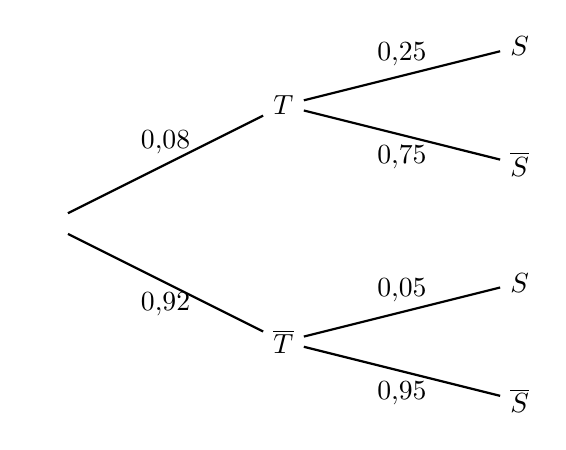
\begin{tikzpicture}[thick, scale=1.5]
\node (P_-1_0) at (-2,-1.5) {$\phantom{A}$};
\node (P_0_0) at (0,-0.5) {$T$};
\draw (P_-1_0) -- (P_0_0) node[midway, above] {$0{,}08$};
\node (P_1_0) at (2,-0) {$S$};
\draw (P_0_0) -- (P_1_0) node[midway, above] {$0{,}25$};
\node (P_1_1) at (2,-1) {$\overline{S}$};
\draw (P_0_0) -- (P_1_1) node[midway, below] {$0{,}75$};
\node (P_0_2) at (0,-2.5) {$\overline{T}$};
\draw (P_-1_0) -- (P_0_2) node[midway, below] {$0{,}92$};
\node (P_1_2) at (2,-2) {$S$};
\draw (P_0_2) -- (P_1_2) node[midway, above] {$0{,}05$};
\node (P_1_3) at (2,-3) {$\overline{S}$};
\draw (P_0_2) -- (P_1_3) node[midway, below] {$0{,}95$};
\end{tikzpicture}
\end{center}

\subsection*{3.}

On a :
\begin{itemize}
    \item \(p(\overline{S} \cap T) = p(T \cap \overline{S}) = p(T) \times p_T(\overline{S}) = 0{,}08 \times 0{,}75 = 0{,}06\).
    \item \(p(\overline{S} \cap \overline{T}) = p(\overline{T} \cap \overline{S}) = p(\overline{T}) \times p_{\overline{T}}(\overline{S}) = 0{,}92 \times 0{,}95 = 0{,}874\).
\end{itemize}

D'après la loi des probabilités totales :
\begin{align*}
p(\overline{S}) &= p(\overline{S} \cap T) + p(\overline{S} \cap \overline{T}) \\
&= 0{,}06 + 0{,}874 \\
&= 0{,}934.
\end{align*}

\subsection*{4.}

\paragraph{a.}
\[
\begin{array}{|c|c|c|c|}
\hline
x_i & 0 & 9 & 14 \\
\hline
P(X = x_i) & 0{,}066 & 0{,}06 & 0{,}874 \\
\hline
\end{array}
\]

\paragraph{b.} Le prix de vente moyen d'un jeu fabriqué par cette entreprise est égal à l'espérance mathématique de la variable aléatoire \(X\), soit :
\[
E(X) = 0 \times 0{,}066 + 9 \times 0{,}06 + 14 \times 0{,}874 = 12{,}776,
\]
soit \( 12{,}78 \) € au centime près.

